\chapter{Definite Integrals}

Integrals are a fundamental concept in calculus. They are used to
calculate areas, volumes, and many other things. A definite integral
calculates the net area between the function and the x-axis over a
given interval.

Recall that you can use a Riemann sum to estimate the area under a 
function, and that as we increase the number of subintervals, the 
estimated area approaches the actual area. In sigma notation we can 
express a Riemann sum as $$\sum_{i=1}^{n} f(x_i)\Delta x$$

\section{Definition}

The definite integral of a function $f(x)$ over an interval $[a, b]$
is defined as the limit of a Riemann sum as $n$ approaches $\infty$:

\begin{equation}
\int_{a}^{b} f(x) \, dx = \lim_{{n \to \infty}} \sum_{i=1}^{n} 
f(x_i^*) \Delta x
\end{equation}

where $x_i^*$ is a sample point in the $i^{th}$ subinterval of a
partition of $[a, b]$, $\Delta x = \frac{b-a}{n}$ is the width of each
subinterval, and the limit is taken as the number of subintervals $n$
approaches infinity.

\begin{Exercise}[label=defint1]
Express $$\lim_{n \to \infty} \sum_{i=1}^{n} (x_i^3 + x_i\sin{x_i})
\Delta x$$ as an integral on the interval $[0, \pi]$. 
\end{Exercise}

\begin{Answer}[ref=defint1]
Following the structure shown in the formal definition of a definite 
integral, we can set $f(x) = x^3 + x\sin{x}$ and rewrite the limit of 
the sum as $\lim_{n \to \infty} \Sigma_{i=1}^{n} f(x)\Delta x = 
\int_{0}^{\pi} f(x)\,dx$. Therefore, the full definite integral 
would be written as $\int_{0}^{\pi} (x^3 + x\sin{x})\, dx$. 
\end{Answer}

\section{Positive and Negative Areas}
What if the function dips below the $x$-axis? We consider that area 
negative. In other words, it represents a \textit{decrease} as opposed to 
an increase. Consider an oscillating object where $v(t) = 
\sin{\pi x}$ (figure \ref{fig:oscillate}). From $t = 0$ to $t = 1$, 
the velocity is positive, which means the object is moving 
\textit{away from} the starting position. This is a positive 
displacement. From $t = 1$ to $t = 2$, the velocity is negative. What 
does this tell you about the direction the object is moving and its 
displacement during this time period? A negative velocity means the 
object is moving \textit{back towards} the starting position.

In general, areas above the $x$-axis are positive, while areas below 
the $x$-axis are negative.

\begin{figure}[htbp]
	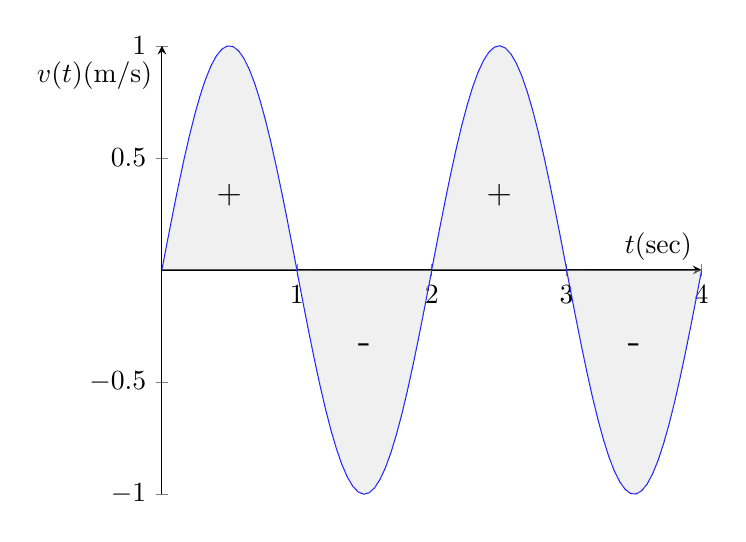
\begin{tikzpicture}
		\begin{axis}
		[xmin=0, xmax=4, ymin=-1, ymax=1, 
		xlabel=$t$(sec), ylabel=$v(t)$(m/s), 
		axis lines = center, ylabel style={yshift=-2.5ex,anchor=east}]
		\addplot[blue, samples=100, domain=0:4]{sin(pi*deg(x))};
        \fill [gray!30, opacity=0.4, domain=0:1, variable=\x]
      		(0, 0)
     		 -- plot ({\x}, {sin(pi*deg(\x))})
      		-- cycle;
      	\node[font=\large] at (0.5, 0.333) {+};
     	\fill [gray!30, opacity=0.4, domain=1:2, variable=\x]
      		(1, 0)
      		-- plot ({\x}, {sin(pi*deg(\x))})
      		-- cycle;
      	\node[font=\Large] at (1.5, -0.333) {-};
      	\fill [gray!30, opacity=0.4, domain=2:3, variable=\x]
      		(2, 0)
      		-- plot ({\x}, {sin(pi*deg(\x))})
      		-- cycle;
      	\node[font=\large] at (2.5, 0.333) {+};
      	\fill [gray!30, opacity=0.4, domain=3:4, variable=\x]
      		(3, 0)
      		-- plot ({\x}, {sin(pi*deg(\x))})
      		-- cycle;
      	\node[font=\Large] at (3.5, -0.333) {-};
		\end{axis}
	\end{tikzpicture}
	\caption{velocity of an oscillating object}
	\label{fig:oscillate}
\end{figure}

\section{Properties of Integrals}
There are several important properties of integrals that will help us 
evaluate more complex integrals in the future. The following examples 
apply when $f(x)$ is continuous or has a finite number of jump 
discontinuities on the interval $a \leq x \leq b$:

\subsection{What happens when $a=b$?}

What if the endpoints of the integral are the same? Let's consider 
$\int_a^b x^2\,dx$, and take the limit as $b \to a$ (shown in figure 
\ref{fig:aequalb}). As you can see, as $b$ approaches $a$, the 
calculated area decreases. Intuitively, we can guess that when $b=a$, 
then the width of the area ($\Delta x$) is zero, and therefore the 
area is also zero. Let's prove this formally. 

Recall that $\int_a^b f(x)\,dx = \lim_{n\to \infty} \sum_{i = 1}^{n}
f(x_i)\Delta x$, where $\Delta x = \frac{b - a}{n}$ and $x_i = a + i
\Delta x$. To evaluate the integral when $b = a$, we will take the 
limit of the limit: $$\lim_{b \to a} \lim_{n \to \infty}f(x_i)
\frac{b - a}{n}$$ This can be rewritten as $$\lim_{b \to a} (b - a) 
\lim_{n \to \infty}\frac{f(x_i)}{n}$$ We know that $\lim_{b \to a}
(b - a) = (a - a) = 0$, and therefore $$\int_a^a f(x)\,dx = 0 \cdot 
\lim_{n \to \infty}\frac{f(x_i)}{n} = 0$$ This is true for any 
function. 

\begin{figure}[htbp]
    \centering
    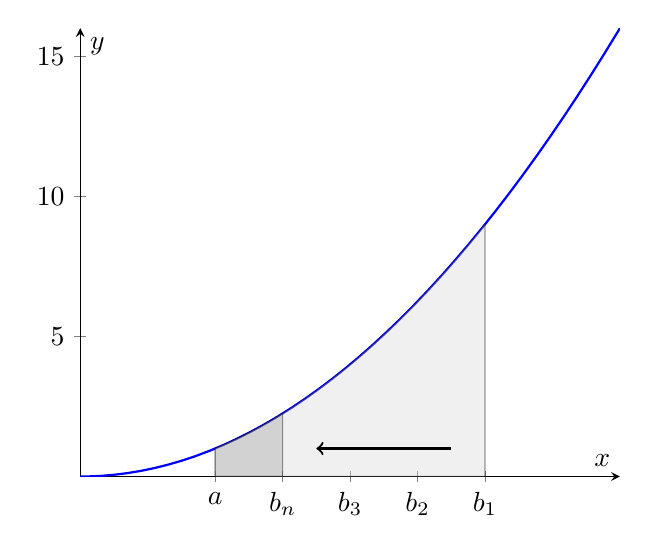
\begin{tikzpicture}
        \begin{axis}[axis lines = center, xmin = 0, xmax = 4, 
        xlabel = $x$, ymin = 0, ymax = 16, ylabel=$y$, 
        xtick={1, 1.5, 2, 2.5, 3}, 
        xticklabels = {$a$, $b_n$, $b_3$, $b_2$, $b_1$}]
            \addplot[blue, thick, samples = 100]{x^2};
            \filldraw[fill=gray!30, opacity=0.4, domain = 1:3, 
            variable=\x]
            (1,0) -- plot ({\x}, {\x*\x}) --(3, 0) -- cycle;
            \filldraw[fill=gray!70, opacity=0.4, domain = 1:1.5, 
            variable=\x]
            (1,0) -- plot ({\x}, {\x*\x}) --(1.5, 0) -- cycle;
            \draw[->, thick](2.75, 1) --(1.75, 1);
        \end{axis}
    \end{tikzpicture}
    \caption{As $b$ gets closer to $a$, the area represented by the 
    integral decreases}
    \label{fig:aequalb}
\end{figure}

\subsection{The integral of a constant}
When the function we are integrating is a constant (that is, it takes 
the form $f(x) = C$), the area is simply $(b - a) \cdot C$. This is 
shown graphically in figure \ref{fig:constant}. 

\begin{figure}[htbp]
	\centering
    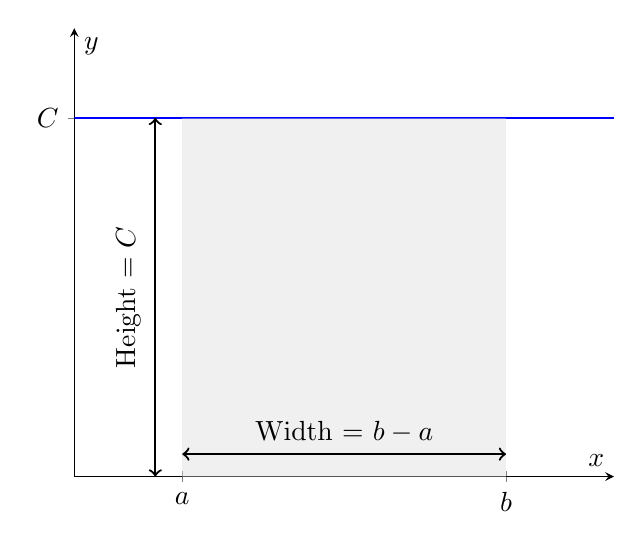
\begin{tikzpicture}
        \begin{axis}[axis lines = center, xmin=0, xmax=5,
        ymin = 0, ymax = 5, xtick={1, 4}, xticklabels={$a$, $b$},
        xlabel=$x$, ylabel=$y$, ytick={4}, yticklabels={$C$}]
            \addplot[blue, thick]{4};
            \fill[gray!30, opacity=0.4](1, 0) rectangle (4, 4);
            \draw[<->, thick](1, 0.25)--(4, 0.25);
            \draw[<->, thick](0.75, 0)--(0.75,4);
            \node[] at (2.5, .5) {Width = $b - a$};
            \node[rotate=90] at (0.5, 2) {Height = $C$};
        \end{axis}
    \end{tikzpicture}
    \caption{$\int_a^b f(x)\,dx = (b - a)\cdot C$}
    \label{fig:constant}
\end{figure}

Since $f(x) = C$ is a horizontal line, the area under $f(x)$ is simply 
a rectangle. As you can see in figure \ref{fig:constant}, the width of 
the rectangle is $b - a$ and the height is $C$. To find the area of a 
rectangle, we multiply the width by the height, and therefore $\int_a^b 
C\,dx = (b - a)\cdot C$.

\subsection{The integral of a function multiplied by a constant}
How is $\int_a^b f(x)\,dx$ related to $\int_a^b C \cdot f(x)\,dx$? 
Intuitively, we know that multiplying a function by a constant, $C$, 
vertically stretches the graph by a factor of $C$. In turn, the area 
under the curve increases by a factor of $C$. Imagine a simple shape, 
like a triangle. If we keep the base of the triangle the same 
(analogous to the integral being over the same interval) and make the 
triangle three times taller (analogous to multiplying the function 
we're integrating by a factor of $C = 3$), then we would expect the 
total area of the triangle to be 3 times greater. Therefore, 
$\int_a^b C \cdot f(x)\,dx = C \int_a^b f(x)\,dx$. 

\subsection{Integrals of sums and differences of functions}
If a function can be described as a sum of two other functions, then 
the integral of the original function is the same as the sum of the 
integrals of the two other functions. Concretely, we say $\int_a^b 
f(x) + g(x)\,dx = \int_a^b f(x)\,dx + \int_a^b g(x)\,dx$. Figure 
\ref{fig:intsum} shows $f(x) = x + 2$, $g(x) = 4x^3-12x^2+10x$, and 
$f(x) + g(x)$. As you can see, the area under $f(x) + g(x)$ is equal 
to the area under $f(x)$ (the red area) plus the area under $g(x)$ 
(the diagonal lined area). 

\begin{figure}[htbp]
    \centering
    \begin{tikzpicture}
        \begin{axis}[axis lines = center, xmin = 0, xmax = 2, 
        xlabel = $x$, ymin = 0, ymax = 8, ylabel = $y$, 
        legend pos = north west]
            \addplot[red, thick, samples=50, domain = 0:2]{x+2};
            \fill[red!30, opacity = 0.4, variable = \x]
            (0,0) -- 
            plot ({\x}, {\x + 2}) --
            (2, 0) -- 
            cycle;
            \addlegendentry{$f(x)$}
            \addplot[blue, thick, samples=50, domain = 0:2]
            {4*x^3-12*x^2+10*x};
            \fill[pattern = north west lines, pattern color = black, 
            variable = \x, domain = 0:2]
            (0,0) -- 
            plot({\x}, {4*\x^3-12*\x^2+10*\x}) -- 
            (2, 0) --
            cycle;
            \addlegendentry{$g(x)$}
            \addplot[violet, thick, samples=50, domain = 0:2]
            {4*x^3-12*x^2+11*x+2};
            \fill[pattern color = black, pattern = north west lines, 
            domain = 0:2, variable = \x] 
            (0,2) -- 
            plot ({\x}, {4*\x^3 - 12*\x^2 + 11*\x + 2}) -- 
            (2, 4) -- 
            plot ({\x}, {\x+2}) -- cycle;
            \addlegendentry{$f(x) + g(x)$}
        \end{axis} 
    \end{tikzpicture}
    \caption{The intergral of $f(x) + g(x)$ is equal to the integral 
    of $f(x)$ plus the integral of $g(x)$}
    \label{fig:intsum}
\end{figure}

Mathematically, we can prove this by recalling that the limit of a 
sum is the sum of the limits: $$\int_a^b f(x) + g(x)\,dx = 
\lim_{n \to \infty} \sum_{i=1}^n [f(x_i)+g(x_i)]\Delta x$$ 
$$=\lim_{n \to \infty} [\sum_{i=1}^n f(x_i)\Delta x + \sum_{i = 1}^n 
g(x_i) \Delta x]$$ $$= \lim_{n \to \infty}\sum_{i=1}^n f(x_i)\Delta 
x + \lim_{n \to \infty} \sum_{i = 1}^n g(x_i) \Delta x$$ $$ = 
\int_a^b f(x)\,dx + \int_a^b g(x)\,dx$$

Similar to the addition property, the integral of the difference 
between two function is equal to the difference of the integrals of 
two functions. $$\int_a^b [f(x) - g(x)]\,dx = \int_a^b f(x)\,dx - 
\int_a^b g(x)\,dx$$. This is more difficult to visualize than addition, 
but we can easily prove it by applying the constant multiple and 
addition properties. Let's define $f(x) - g(x) = f(x) + (-g(x))$: 
$$\int_a^b f(x) - g(x)\,dx = \int_a^b f(x) + (-g(x))\,dx$$\\
By the addition property, $$=\int_a^b f(x)\,dx + \int_a^b -g(x)\,dx = 
\int_a^b f(x)\,dx + \int_a^b (-1)\cdot g(x)\,dx$$\\
By the constant multiple property: $$=\int_a^b f(x)\,dx - \int_a^b 
g(x)\,dx$$

\subsection{Integrals of adjacent areas}
If $c$ is some $x$-value between $a$ and $b$, then $\int_a^c f(x)\,dx 
+ \int_c^b f(x)\,dx = \int_a^b f(x)\,dx$. This is shown graphically in 
figure \ref{fig:adjacent}. The total area from $x=a$ to $x=b$ is equal 
to the red area (the integral from $a$ to $c$) plus the blue area (the 
integral from $c$ to $b$). 

\begin{figure}[htbp]
	\centering
	\begin{tikzpicture}
		\begin{axis}
		[axis lines = center, xmin = 0, xmax = 2, xlabel = $x$, 
		ymin = 0, ymax = 8, ylabel = $y$,
		xtick = {0.5, 1, 1.5, 2}, xticklabels = {$a$, $c$, $b$ , }]
		\addplot[blue, thick, domain = 0:2]{4*x^3-12*x^2+11*x+2};
		\fill[blue!30, opacity = 0.4, variable = \x, domain = 0.5:1]
		(0.5,0) -- 
		plot({\x},{4*\x^3 - 12*\x^2 + 11*\x + 2}) -- 
		(1,0) -- 
		cycle;
		\fill[red!30, opacity = 0.4, variable = \x, domain = 1:1.5]
		(1, 0) --
		plot ({\x}, {4*\x^3 - 12*\x^2 + 11*\x + 2})--
		(1.5, 0)--
		cycle;
		\fill[pattern = north west lines, variable = \x, domain = 0.5:1.5]
		(0.5, 0) --
		plot ({\x}, {4*\x^3 - 12*\x^2 + 11*\x + 2})--
		(1.5, 0)--
		cycle;
		\end{axis}
	\end{tikzpicture}
	\caption{$\int_a^c f(x)\,dx + \int_c^b f(x)\,dx = \int_a^b f(x)\,dx$}
	\label{fig:adjacent}
\end{figure}

\subsection{Estimating the value of an integral}
Suppose we need to know the area under a complex function. We can 
estimate a range for the value of the integral if we can bookend the 
function over the interval we are interested. Suppose there is some 
value $m$ such that $f(x) \geq m$, and some other value $M$ such that 
$f(x) \leq M$ on the interval we are interested in (see figure 
\ref{fig:bookend}). The total area under $f(x)$ is the light blue 
plus the darker blue. The total area under $y=M$ is the darker blue, 
plus the light blue, plus the white area. The darker blue area under 
the curve has total area $m \cdot (b - a)$ and the rectangle under 
$y=M$ has total area $M \cdot (b - a)$ (since these are both integrals 
of a constant, which we learned about above). The actual area under our 
function is more than just the dark blue area, but less than the total 
area under $y=M$. Therefore, $m(b - a) \leq \int_a^b f(x)\,dx \leq 
M(b -a)$ if $m \leq f(x)$ and $M \geq f(x)$ on the interval $x \in 
[a, b]$. 

\begin{figure}[htbp]
	\centering
	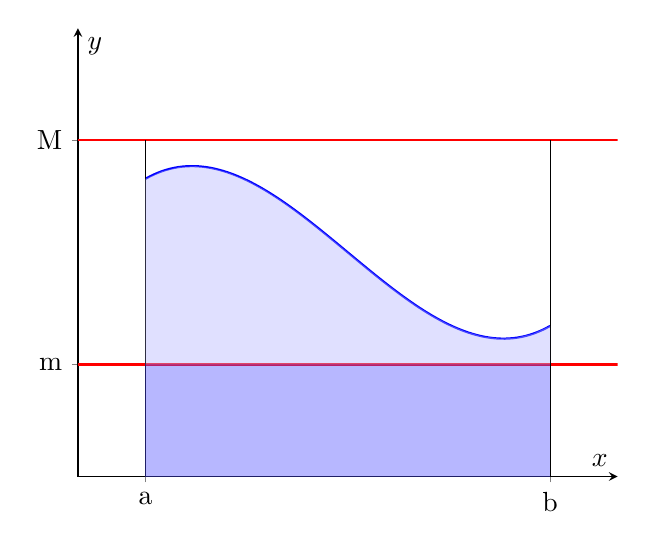
\begin{tikzpicture}
		\begin{axis}[axis lines = center, xmin = 0, xmax = 2, xlabel = $x$,
		xtick={0.25, 1.75}, xticklabels = {a, b},
		ymin = 0, ymax = 2, ylabel = $y$, ytick = {0.5, 1.5}, 
		yticklabels={m, M}]
			\addplot[blue, thick, domain = 0.25:1.75, samples = 100]
			{(x)*(x-1)*(x-2)+1};
			\addplot[red, thick, domain = 0:2]{0.5};
			\addplot[red, thick, domain = 0:2]{1.5};
			\addplot[black]coordinates{(0.25, 0) (0.25, 1.5)};	
			\addplot[black]coordinates{(1.75, 0) (1.75, 1.5)};	
			\fill[blue!70, opacity = 0.4] (0.25, 0) rectangle (1.75, 0.5);
			\fill[blue!30, opacity = 0.4, domain =0.25:1.75] (0.25, 0.5) -- 
			plot ({\x}, {(\x)*(\x-1)*(\x-2)+1}) -- (1.75, 0.5) --cycle;
		\end{axis}
	\end{tikzpicture}
	\caption{$m \leq f(x) \leq	M$}
	\label{fig:bookend}
\end{figure}

\subsection{Other Properties of Integrals}
If $f(x) \geq 0$ over the for $a \leq x \leq b$, then $\int_a^b 
f(x)\,dx >0$. We can make an intuitive, geometric argument to support 
this claim. Recall that areas above the $x$-axis are considered 
positive. If $f(x) \geq 0$, then all the area of the integral lies 
above the $x$-axisj therefore, the total area must be positive. 

Similarly, if $f(x) \geq g(x)$ on the interval $a \leq x \leq b$, 
then $\int_a^b f(x)\,dx \geq \int_a^b g(x)\,dx$ (see figure 
\ref{fig:compare}). The entire area under $g(x)$ is contained in the 
area under $f(x)$. Therefore, $\int_a^b f(x)\,dx \geq \int_a^b 
g(x)\,dx$

\begin{figure}[htbp]
	\centering
	\begin{tikzpicture}
		\begin{axis}[xmin=0, xmax = 3.5, xlabel=$x$, xtick={0.25, 3.392}, 
		xticklabels={$a$, $b$}, ymin = 0, ymax = 3.5, ylabel=$y$, 
		axis lines = center, legend pos = north west]
			\addplot[red, thick, samples = 50, domain = 0.25:3.392]{x - 0.25};
			\addlegendentry{$f(x)$}
			\fill[pattern = north west lines, pattern color = red!30, 
			domain = 0.25:3.392, variable = \x]
			(0.25, 0) -- 
			plot({\x},{\x - 0.25}) -- 
			(3.392, 0) -- 
			plot({\x},{sin(deg(\x - 0.25))}) -- 
			cycle;
			\addplot[blue, thick, samples = 100, domain = -.25:3.392]
			{sin(deg(x - 0.25))};
			\addlegendentry{$g(x)$}
			\fill[blue!30, opacity = 0.4, domain = 0.25:3.392, variable = \x]
			(0.25, 0) -- 
			plot({\x},{sin(deg(\x - 0.25))}) -- 
			(3.392, 0) -- 
			cycle;
		\end{axis}
	\end{tikzpicture}
	\caption{$\int_a^b f(x)\,dx \geq \int_a^b g(x)\,dx$}
	\label{fig:compare}
\end{figure}

Lastly, we see what happens when we switch $a$ and $b$. While it is 
unusual to integrate from right to left (that is, in a case where 
$a > b$), this property will be useful. Recall that $$\int_a^b f(x)\,dx 
= \lim_{n \to \infty} \sum_{i = 1}^{n} f(x_i)\frac{(b - a)}{n}$$\\ 
What is $\int_b^a f(x)\,dx$? Substituting, we see that $$\int_b^a f(x)
\,dx =\lim_{n \to \infty} \sum_{i=1}^{n} f(x_i) \frac{(a - b)}{n}$$\\ 
Noting that $(a - b) = -(b - a)$ we see: $$\int_b^a f(x)\,dx = \lim_{n \to 
\infty} \sum_{i = 1}^{n} f(x_i) \frac{-(b - a)}{n}$$ $$=(-1)\lim_{n 
\to \infty} \sum_{i = 1}^{n} f(x_i) \frac{(b - a)}{n}$$ $$=(-1)
\int_a^b f(x)\,dx$$ \\
Therefore, it is true that $\int_b^a f(x)\,dx = -\int_a^b f(x)\,dx$. 

\section{Applications in Physics}
We have already seen that the area under a velocity function is 
displacement, and the area under an acceleration function is change in 
velocity (Riemann Sums). We can use integrals to determine the change 
in position of an object over a given time frame. If we \textit{also} 
know the object's starting position, then we can state the object's 
ending position. Consider the graph of an object's velocity in figure 
\ref{fig:velocity}:

\begin{figure}[htbp]
	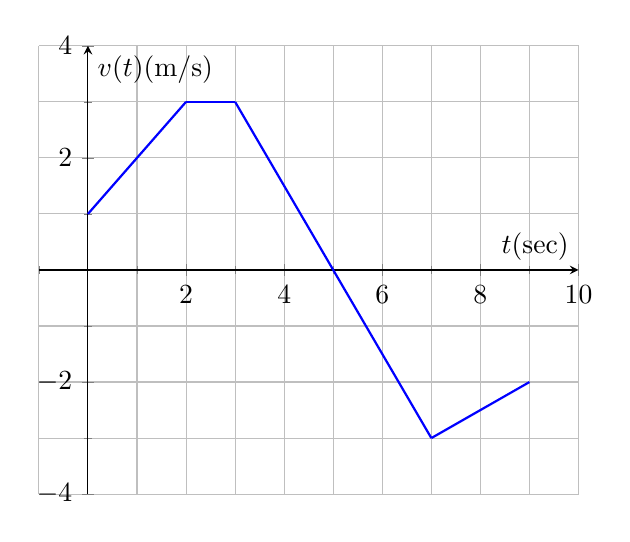
\begin{tikzpicture}
		\begin{axis}[axis lines = center, 
		xmin=-1, xmax=10, ymin=-4, ymax=4, 
		xlabel=$t$(sec), ylabel=$v(t)$(m/s), 
		xtick={}, ytick={}, grid=both, minor tick num = 1]
		\addplot[blue, thick] coordinates {(0, 1) (2, 3)};
		\addplot[blue, thick] coordinates {(2, 3) (3, 3)};
		\addplot[blue, thick] coordinates {(3, 3) (7, -3)};
		\addplot[blue, thick] coordinates {(7, -3) (9, -2)};
		\end{axis}
	\end{tikzpicture}
	\caption{Velocity of an object from $t=0$ to $t=9$}
	\label{fig:velocity}
\end{figure}

We can determine the net displacement of the object from $t = 0$ to 
$t = 9$ by evaluating $\int_{0}^{9} v(t)\, dt$. Since the definite 
integral is equal to the area under the curve, we need to find the 
total area. As the function consists of straight lines, we will leave 
the explicit calculation of the area as an exercise for the student. 
You should find that the total positive area (above the $x$-axis) is 
10 meters, and the total negative area (below the $x$-axis) is 8 meters. 
Therefore, the object's displacement over the specified time interval 
is $10 - 8 = 2$ meters. 

When you push on something to move it, you are applying a force over 
a distance (assuming you are strong enough to move it!). The integral 
of force as a function of distance is the \textit{work} done on that 
object.  Work is the change in kinetic energy (KE) of an object. 
Mathematically, this is $$\int_{a}^{b} F(x)\,dx = \Delta KE = 
\frac{1}{2} m (v_f^2 - v_i^2)$$.

If you integrate the force as a function of time, that is 
\textit{impulse}. Impulse is the change in momentum (p) of the 
object. Mathematically, this is $$\int_{a}^{b} F(t)\,dt = \Delta p 
= m (v_f - v_i)$$.

Example problem: You push a 3 kg box with force $F(x) = 0.5x$, where 
$x$ is measured in meters and $F$ is measured in Newtons. If the box 
was initially at rest, what is its speed when it reaches the 2 meter 
mark? (Hint: $KE = \frac{1}{2} m v^2$.) 

Solution: Change in kinetic energy is the area under a force-distance 
curve. We can plot the force applied to the box from d=0 to d=2 (see 
figure \ref{fig:KEbox}):

\begin{figure}[htbp]
	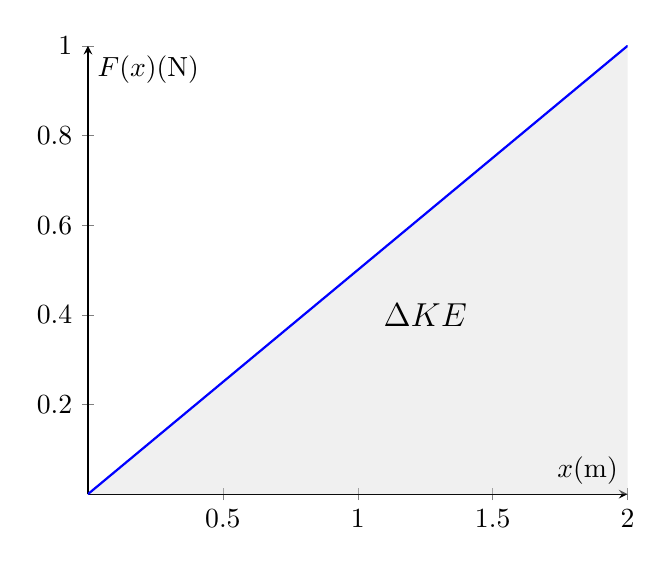
\begin{tikzpicture}
		\begin{axis}
		[xmin=0, xmax=2, ymin=0, ymax=1, 
		xlabel=$x$(m), ylabel=$F(x)$(N), axis lines = center]
            \fill[gray!30, opacity=0.4](0,0) --(2, 0) -- (2,1) -- cycle;
            \node[font=\large] at (1.25, 0.4) {$\Delta KE$};
		\addplot[blue, thick]{0.5*x};
		\end{axis}
	\end{tikzpicture}
 \caption{Force applied to a box over a distance; the shaded area 
 represents the change in kinetic energy.}
 \label{fig:KEbox}
\end{figure}

Given that the box's initial velocity is $0 \frac{m}{s}$, we know that 
the initial kinetic energy (KE) is $0J$. This implies that $KE_f = 
\Delta KE$. We can find $\Delta KE$ from the shaded area:\\
$$\Delta KE = \frac{1}{2} (2m) (1N) = 1 J = KE_f$$\\
Solving for the final velocity:\\
$$KE_f = 1 J = \frac{1}{2}(3kg)(v^2)$$
$$2 J = (3 kg) (v^2)$$
$$\frac{2}{3} \frac{m^2}{s^2} = v^2$$
$$v=\sqrt{\frac{2}{3} \frac{m^2}{s^2}} \approx 0.816 \frac{m}{s}$$


\section{Practice Exercises}
\begin{Exercise}[label=defint2]
Given that $\int_{0}^{1} x^2\,dx = \frac{1}{3}$, use the properties 
of integrals to evaluate $\int_{0}^{1} (5-6x^2)\,dx$. 
\end{Exercise}

\begin{Answer}[ref=defint2]
By property 6, we know that $$\int_{0}^{1} (5-6x^2)\,dx = \int_{0}^{1} 
5\,dx - \int_{0}^{1} 6x^2\,dx$$\\
By property 5, we know that $$\int_{0}^{1} 5\,dx - \int_{0}^{1} 6x^2\,
dx = \int_{0}^{1} 5\,dx - 6\int_{0}^{1} x^2\,dx$$\\
By property 3, we know that $$\int_{0}^{1} 5\,dx = 5(1 - 0) = 5$$\\
Putting it all together, we see that $$\int_{0}^{1} (5-6x^2)\,dx = 5 
- 6(\frac{1}{3}) = 5 - 2 = 3$$
\end{Answer}

\begin{Exercise}[label=defint3]
	This question was originally presented as a multiple-choice problem 
	on the 2012 AP Calculus BC exam. The graph of $f$ is shown. What is 
	the value of $\int_{0}^{4} f(x)\,dx$?\\
	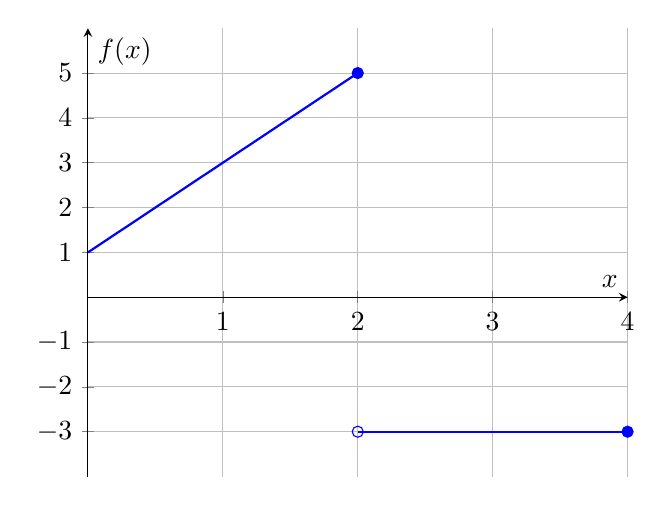
\begin{tikzpicture}
		\begin{axis}
		[xmin=0, xmax=4, xlabel=$x$, 
		ylabel=$f(x)$, ymin = -4, ymax=6, 
		axis lines = center, minor tick = 1, grid = major, 
		ytick={-3, -2, -1, 1, 2, 3, 4, 5}]
		      \addplot[blue, thick]coordinates{(0, 1) (2, 5)};
		      \addplot[mark=*, blue]coordinates{(2, 5)};
		      \addplot[mark=o, blue]coordinates{(2, -3)};
		      \addplot[blue, thick]coordinates{(2, -3) (4, -3)};
    		\addplot[mark=*, blue]coordinates{(4, -3)};
		\end{axis}
	\end{tikzpicture}
\end{Exercise}

\begin{Answer}[ref=defint3]
We can break the integral into two parts: from $x = 0$ to $x = 2$ 
(shaded in blue), and from $x = 2$ to $x = 4$ (shaded in red). The 
blue portion is a trapezoid, so it has a total area of $\frac{1}{2} 
(b_1 + b_2) (h) = \frac{1}{2} (1 + 5) (2) = 6$. Because it is above 
the $x$-axis, the area is positive. The red portion is a rectangle and 
has a total area of $2 \times 3 = 6$ and is \textit{negative}, because 
it lies below the $x$-axis. Therefore, the total area is $6 + -6 = 0$. \\

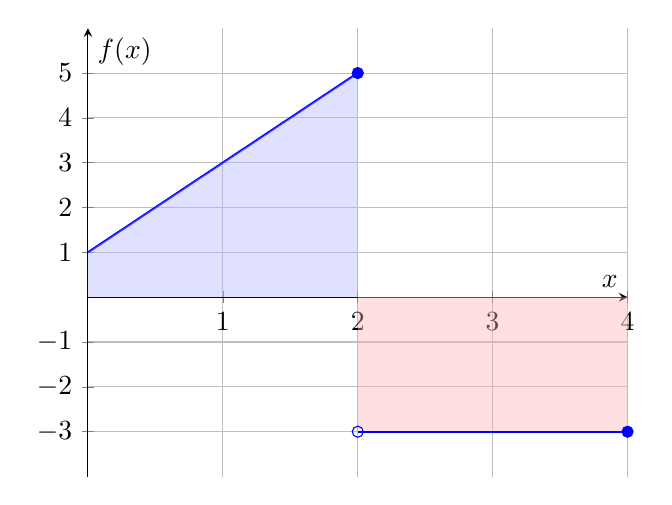
\begin{tikzpicture}
		\begin{axis}
		[xmin=0, xmax=4, xlabel=$x$, 
		ylabel=$f(x)$, ymin = -4, ymax=6, 
		axis lines = center, minor tick = 1, grid = major, 
		ytick={-3, -2, -1, 1, 2, 3, 4, 5}]
		      \addplot[blue, thick]coordinates{(0, 1) (2, 5)};
		      \fill[blue!30, opacity=0.4](0, 0)--(2, 0)--(2, 5)--(0,1)--cycle;
		      \fill[red!30, opacity=0.4](2, 0) rectangle (4, -3);
		      \addplot[mark=*, blue]coordinates{(2, 5)};
		      \addplot[mark=o, blue]coordinates{(2, -3)};
		      \addplot[blue, thick]coordinates{(2, -3) (4, -3)};
    		\addplot[mark=*, blue]coordinates{(4, -3)};
		\end{axis}
	\end{tikzpicture}
\end{Answer}

\begin{Exercise}[label=defint4]
	This question was originally presented as a multiple-choice problem 
	on the 2012 AP Calculus BC exam. The graph of the piecewise function 
	$g(x)$ is shown. What is the value of $\int_{-1}^{9} 3 g(x) + 2\,dx$?
	
	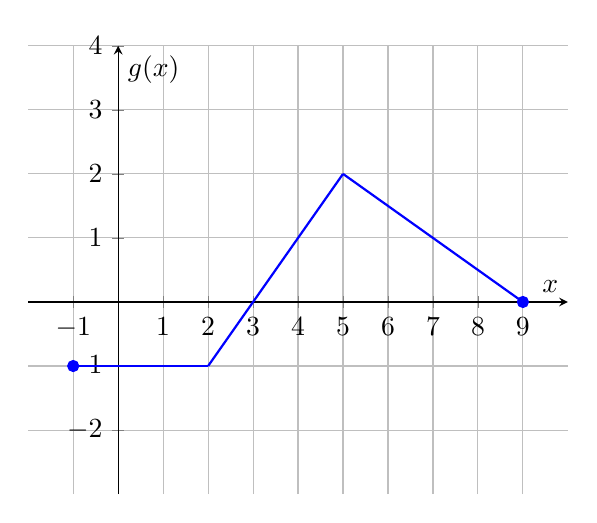
\begin{tikzpicture}
		\begin{axis}
		[xmin=-2, xmax=10, ymin=-3, ymax=4, 
		axis lines = center, xlabel=$x$, ylabel=$g(x)$, 
		grid=major, ytick={-2, -1, 1, 2, 3, 4}, xtick={-1, 1, 2, 3, 4, 5, 6, 7, 8, 9}]
		\addplot[blue, thick]coordinates{(-1, -1) (2, -1)};
		\addplot[blue, thick]coordinates{(2, -1) (5, 2)};
		\addplot[blue, thick]coordinates{(5, 2) (9, 0)};
            \addplot[blue, mark=*, only marks]coordinates{(-1, -1) (9, 0)};
		\end{axis}
	\end{tikzpicture}
\end{Exercise}

\begin{Answer}[ref=defint4]
Using the properties of integrals, we can rewrite $\int_{-1}^{9} 3 
g(x) + 2\,dx$ as $3 \int_{-1}^{9} g(x)\,dx + 2 (9-(-1))$. From the 
graph, we can determine $\int_{-1}^{9} g(x)\,dx = 2.5$. Therefore, 
$\int_{-1}^{9} 3 g(x) + 2\,dx = 3 (2.5) + 2 (10) = 27.5$. 
\end{Answer}

\begin{Exercise}[label = defint5]
[This question was originally presented as a calculator-allowed, multiple-
choice question on the 2012 AP Calculus BC exam.] If $f'(x) > 0$ for all real 
numbers and $\int_4^7 f(x)\,dx = 0$, which of the following could be a table 
of values for the function $f$?\\
(A) \begin{tabular}{|c|c|}\hline
$x$ & $f(x)$\\\hline
4 & -4\\\hline
5 & -3\\\hline
7 & 0\\\hline
\end{tabular}
(B)\begin{tabular}{|c|c|}\hline
$x$ & $f(x)$\\\hline
4 & -4\\\hline
5 & -2\\\hline
7 & 5\\\hline
\end{tabular}
(C)\begin{tabular}{|c|c|}\hline
$x$ & $f(x)$\\\hline
4 & -4\\\hline
5 & 6\\\hline
7 & 3\\\hline
\end{tabular}
(D)\begin{tabular}{|c|c|}\hline
$x$ & $f(x)$\\\hline
4 & 0\\\hline
5 & 0\\\hline
7 & 0\\\hline
\end{tabular}
(E)\begin{tabular}{|c|c|}\hline
$x$ & $f(x)$\\\hline
4 & 0\\\hline
5 & 4\\\hline
7 & 6\\\hline
\end{tabular}
\end{Exercise}

\begin{Answer}[ref = defint5]
(B). If $f'(x) > 0$ for all $x$, then $f$ must be increasing for $4 < x < 7$. 
Since (C) decreases from $x = 5$ to $x = 7$, we can eliminate it. We can also 
eliminate (D), since $f(4) = f(5) = f(7)$, which implies either the slope of 
$f$ is zero or changes from positive to negative. If $\int_4^7 f(x)\,dx = $, 
then some portion of $f(x)$ lies above the $x-axis$, while some other portion 
lies below (we must have positive and negative areas for the sum to be zero). 
This eliminates (A) and (E), since the integral of (A) would have a negative 
value and the integral of (E) would have a positive value. This leaves (B). 
\end{Answer}


